\subsection{Arquitectura  del servidor}

El servidor se ha implementado con Spring Boot \cite{spring}, un framework que permite la creación de aplicaciones en Java de una forma más sencilla. Esta simplifica el proceso de gestión de las dependencias, permitiendo que nos centremos lo máximo posible en el desarrollo de la aplicación.

\begin{figure}[H]
\centerline{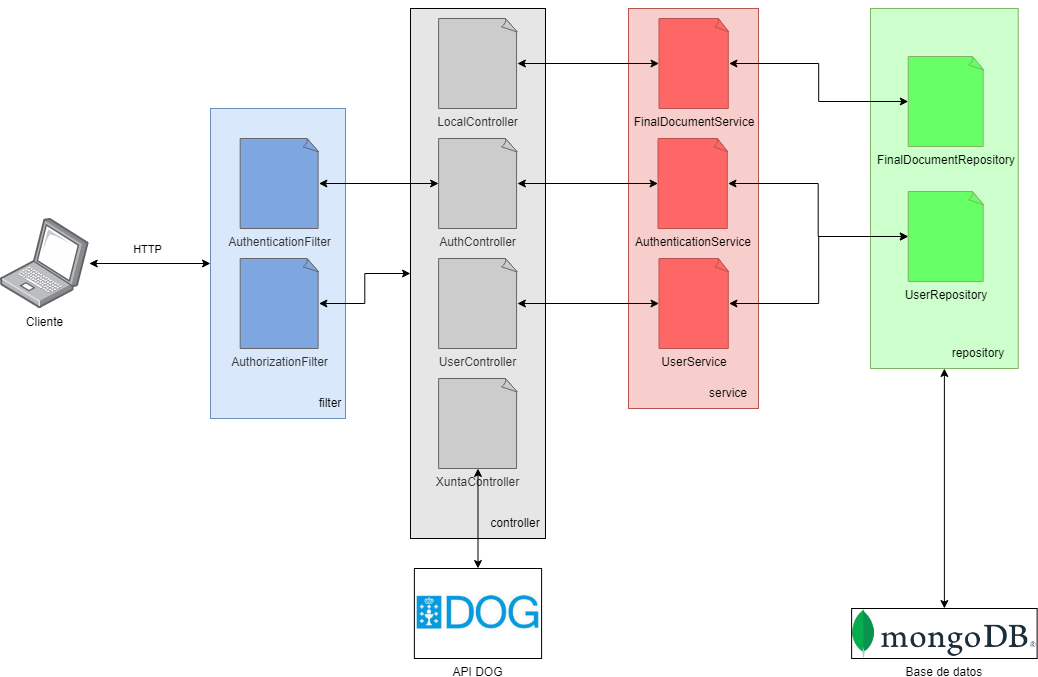
\includegraphics[width=15cm]{figuras/diseño/FicherosServidor.png}}
\caption{Arquitectura del servidor.}
\label{enlaceArquitecturaServidor}
\end{figure}

El servidor está dividido en un conjunto de directorios, cada uno con una función diferente. 
\\

Todas las dependencias del servidor son definidas en el archivo {\bf build.gradle}. Dichas dependencias son tratadas por Gradle \cite{gradle}, un gestor de dependencias en aplicaciones de Java.
\\

En el subdirectorio {\bf main}, encontraremos una carpeta denominada {\bf resources}. En el fichero contenido en ella, se define el nombre de la base de datos que ha de utilizar la aplicación.
\\

Si accedemos al directorio {\bf java/tfg/project}, encontramos el contenido principal del servidor. El archivo {\bf Application} es el encargado de desplegar el servidor, pues contiene la función main del programa.
\\

En el directorio {\bf Config}, se localizan archivos de configuración del propio servidor, tales como aspectos de seguridad, documentación, privacidad, etc. 
\\

Otro directorio es el {\bf Filter}, donde se tratan distintos aspectos de seguridad con respecto a los usuarios que utilizan la aplicación, como puede ser el inicio de sesión, gestión de contraseñas o comprobación de roles.
\\

En la carpeta {\bf Model} encontramos los distintos objetos que conforman la base de la aplicación. Podemos destacar entre ellos el objeto {\bf FinalDocument}, que está formado por todos los atributos de la ley, y {\bf User}, que es el objeto utilizado para gestionar los usuarios. Todos estos objetos son empleados por las clases definidas en las carpetas {\bf Controller, Service y Repository}.
\\

En la carpeta {\bf Controller}, encontramos todos los archivos encargados de redirigir las llamadas a los servicios necesarios en la carpeta Service. Estos se encargan de localizar cualquier llamada al servidor (GET, POST, ...), y entregarla a los servicios.
\\

Con respecto al directorio {\bf Service}, este contiene los archivos donde se localizan los servicios web. Aquí se implementa la lógica de negocio de la aplicación, y no se conserva estado. Es llamada por los controladores, y solicita información a los repositorios donde se almacena toda la información.
\\

Como último directorio, se encuentra {\bf Repository}, donde se almacenan los ficheros que se encargan del acceso y almacenamiento de datos. Estos gestionan la conexión con la base de datos para poder obtener/almacenar información en ella.
\\

En resumen, las funcionalidades de los controladores, servicios y repositorios son las siguientes:
\begin{itemize}
    \item {\bf LocalController, FinalDocumentService y FinalDocumentRepository}: se encargan de gestionar las operaciones relacionadas con las leyes.
    \item {\bf UserController, UserService y UserRepository}: se encargan de gestionar las operaciones relacionadas con los usuarios.
    \item {\bf AuthController, AuthenticationService y UserRepository}: se encargan de gestionar las operaciones relacionadas con aspectos de seguridad respecto a los usuarios, como el inicio de sesión.
    \item {\bf XuntaController}: se encarga de gestionar las llamadas a la API de la Xunta.
\end{itemize}

\subsubsection{Listado de servicios}

Como se ha mencionado anteriormente, el servidor sigue una arquitectura basada en servicios REST, los cuales permiten el acceso a recursos mediante los verbos HTTP. La información completa de dichos servicios se puede consultar en la documentación de la API del servidor en la URI {\it /swagger-ui/index.html}. Por ejemplo, en el caso de desplegar el servidor localmente, el enlace sería {\it \url{http://localhost:8080/swagger-ui/index.html}}.

\begin{figure}[H]
\centerline{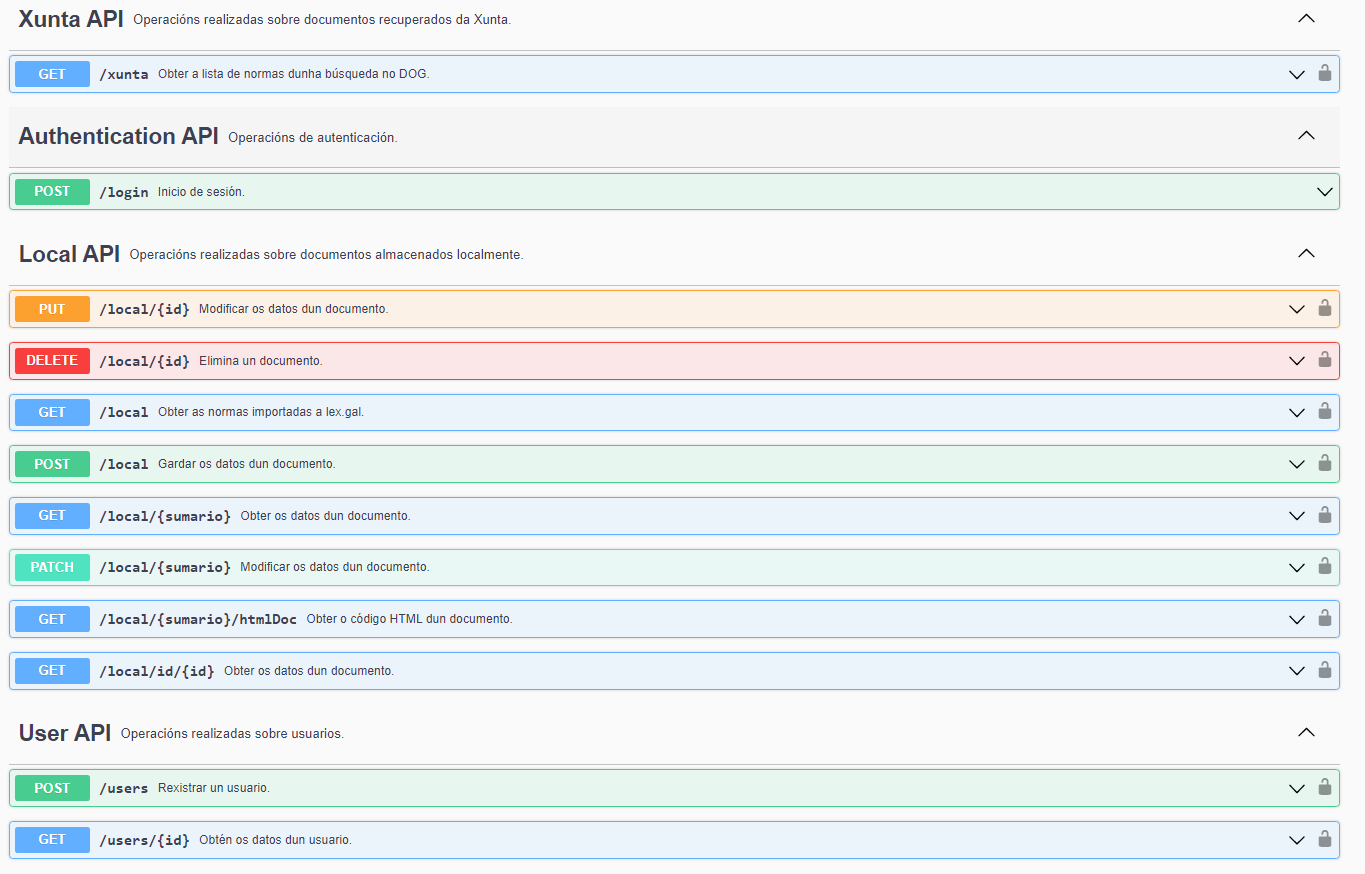
\includegraphics[width=15cm]{figuras/diseño/APIServidor.PNG}}
\caption{API del servidor.}
\label{enlaceAPIServidor}
\end{figure}

Los servicios listados en la \hyperref[enlaceAPIServidor]{Figura 3.3} se pueden resumir en lo descrito a continuación:

\begin{itemize}
    \item {\bf Xunta API}: existe una única operación GET, la cual se encarga de devolver el listado de leyes encontradas en el DOG. Para poder utilizar este servicio, es necesario estar autenticado. La URI de acceso es {\it /xunta}.
    \item {\bf Authentication API}: una única operación también, en este caso un POST. Se encarga de gestionar el inicio de sesión por parte de un usuario, devolviendo un token JWT \cite{jwt} para mayor seguridad ({\bf NFR-10}). Es la única operación donde no es necesario estar autenticado y la URI de acceso es {\it /login}.
    \item {\bf Local API}: se encuentran aquí los servicios más importantes de la aplicación, y por ello tenemos muchos más que en el resto de controladores. Solamente es necesario estar autenticado para poder operar con estos servicios, y se explican a continuación:
        \begin{itemize}
            \item Cuatro servicios GET. El primero de ellos, al cual se accede mediante la URI {\it /local} devuelve todas las leyes encontradas. Hay otros dos ({\it /local/{sumario}} y {\it /local/{id}}) que permiten buscar una ley concreta a partir de su sumario e id respectivamente. Por último, {\it /local/{sumario}/htmlDoc}, que devuelve el documento HTML de una ley.
            \item Un POST para crear objetos de leyes. El contenido del documento de una ley se almacena en formato HTML, cumpliendo con el requisito {\bf NFR-05}. Se accede mediante la URI {\it /local}.
            \item Las operaciones PUT en la URI {\it /local/{id}} y PATCH {\it /local/{sumario}} para modificar los datos de documentos. La operación PUT se utiliza cuando es necesario modificar un documento en su totalidad, mientras que PATCH solo cambia los atributos que es necesario.
            \item El servicio DELETE en la URI {\it /local/{id}}, que se encarga de eliminar una ley de la base de datos.
        \end{itemize}
    \item {\bf User API}: dos operaciones para gestionar usuarios. La primera de ellas es un GET a la URI {\it /users/{id}} para obtener los datos de un usuario, y solo es necesario estar autenticado para obtener dichos datos. La segunda, es un POST a la URI {\it /users}. Esta operación inserta un usuario con la contraseña encriptada ({\bf NFR-02}), así como solo puede ser realizada por usuarios que poseen el rol de administrador ({\bf NFR-03}).
\end{itemize}